\documentclass[12pt]{article}
\usepackage[T1]{fontenc}
\usepackage[utf8]{inputenc}
\usepackage{amssymb}
\usepackage{amsmath}
\usepackage{color}
\usepackage{tikz}

\begin{document}

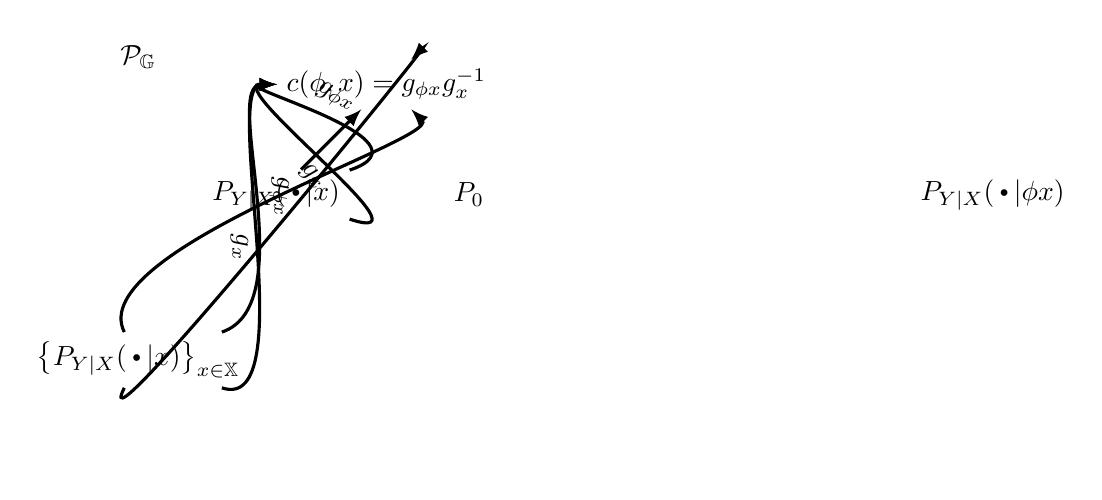
\begin{tikzpicture}[scale=0.7]

\tikzstyle{every node}=[font=\normalsize]

\node at (-3,-1.5) (P0) {$P_0$};
\node at (-6.5,-1.5) (GX) {$P_{Y|X}({\,\vcenter{\hbox{\tiny$\bullet$}}\,}|x)$};
\node at (6.5,-1.5) (GXphi) {$P_{Y|X}({\,\vcenter{\hbox{\tiny$\bullet$}}\,}|\phi x)$};
\node at (-4.5,0.5) (GXphi) {$c(\phi,x)=g_{\phi x}g_x^{-1}$};

\draw[-latex,line width=0.4mm] (GX) -- (GXphi) ;

\node at (-9,1) (PX) {$\mathcal{P}_{\mathbb{G}}$};

\draw[-latex,line width=0.4mm] (GX) .. controls +(3,1) and +(-3,0) .. (GXphi) node [midway,sloped,above] {$g_{\phi x}$} ;
\draw[-latex,line width=0.4mm] (GX) .. controls +(3,-1) and +(-3,0) .. (GXphi) node [midway,sloped,below] {$g_{x}$} ;

\node at (-9,-4.5) (GX) {$\left\{P_{Y|X}({\,\vcenter{\hbox{\tiny$\bullet$}}\,}|x)\right\}_{x\in\mathbb{X}}$};

\draw[-latex,line width=0.4mm] (GX) .. controls +(3,1) and +(-3,0) .. (GXphi) node [midway,sloped,above] {$g_{\phi x}$} ;
\draw[-latex,line width=0.4mm] (GX) .. controls +(3,-1) and +(-3,0) .. (GXphi) node [midway,sloped,below] {$g_{x}$} ;

\draw[-latex,line width=0.4mm] (GX) .. controls +(-1,2) and +(1,-1) .. (GXphi);
\draw[-latex,line width=0.4mm] (GX) .. controls +(-1,-2) and +(1,1) .. (GXphi);

\end{tikzpicture}

\end{document}